\subsection{Bond power and the current-based power form}\label{sec:m-bond}

\emph{Theory.} Bond's third theory of comminution~\cite{bond1952} gives the specific energy of a size reduction from a feed $80\%$
passing size to a product $80\%$ passing size, both in micrometres, through the work index of the ore:
\begin{equation}
W = 10\,W_i\left(\frac{1}{\sqrt{P_{80}}} - \frac{1}{\sqrt{F_{80}}}\right)\ [\mathrm{kWh/t}],\qquad
P_d = \max(0,\ W)\,Q\ [\mathrm{kW}],
\label{eq:bond}
\end{equation}
so the net draw $P_d$ is the specific energy times the throughput of Section~\ref{sec:m-capacity}. On the circuit cases $P_d$ is the
power the engine reports; at S01 it is $287.4$~kW. Bond's law was developed for grinding, and it is known to be a weak descriptor of
coarse crushing duty; Morrell's size-specific energy (Section~\ref{sec:m-morrell}) is the documented alternative and is held out beside
it. On the calibrated lane the engine applies the current-based form that Rocha et al.\ fitted to the HP500~\cite{rocha2024}, reading
the paper's net power as the Bond draw,
\begin{equation}
P_c = \zeta\,P_d + P_n,\qquad \zeta = 1.30,\quad P_n = 110\ \mathrm{kW},
\label{eq:pc}
\end{equation}
with $P_n$ the no-load power. In the paper $P_d$ is a size-specific net power of the paper's own model, not the Bond draw, so the two
constants do not transfer; the backbone document states this in its note.

\emph{What the measured power says.} Table~\ref{tab:power-parity} and Figure~\ref{fig:power-parity} hold the three power estimates of the
calibrated engine against the ten measured values in sample. The bare Bond draw is nearly flat, from $196.1$ to $237.5$~kW, against a
measured spread of $187$ to $355$~kW: its mean absolute percentage error is $26.88\%$ and its $R^2$ is $-1.29$. The published form
overshoots, at $47.58\%$ and $R^2=-3.64$, because its constants are for a different $P_d$. The best the form can do on these data, a
least-squares refit of $\zeta$ and $P_n$ on all ten surveys, reaches $19.28\%$ with $\zeta=-2.41$ and $P_n=828.6$~kW: a negative slope that
collapses the prediction toward the survey mean, which is a fit and not a physical constant. The constant mean itself is at $22.03\%$. Out
of sample the picture is the same (Section~\ref{sec:results-bench}).

\emph{Why the draw is flat.} At S01 the law gives $W=140\,(27{,}698^{-1/2}-126{,}030^{-1/2})=0.447$~kWh/t and, at $643.16$~t/h, the
$287.4$~kW of the trace. On the survey lane the same decomposition explains the flat draw within the model: the specific energy of the
backbone rises as the setting tightens, from $0.190$~kWh/t at $54$~mm (survey 1) to $0.229$~kWh/t at $40$~mm (survey 6), while its throughput
falls from $1208.9$ to $970.5$~t/h, and the product of the two moves only from $229.5$ to $222.5$~kW. The measured power instead rises from
$209$ to $355$~kW between the same two surveys. The engine's power therefore cannot follow the measured power, whatever its two constants, unless
the specific energy rose much faster with a tighter setting than the Bond law and the engine's product sizes make it; whether the plant's
current-based power measures something other than the comminution energy, a no-load share that grows at tight settings for example, cannot be
decided from these data.

\emph{Parameters and how they were set.} $W_i$ is a case input on the circuit cases ($2$ to $40$~kWh/t accepted) and the blend value
$9.0$~kWh/t on the HP500 lane, between the compact ($7.2$) and the supercompact ($10.6$) itabirite bands carried from the source; $\zeta$
and $P_n$ are the published values, refit per fold by CrusherCal and sampled by CrusherBayes. The draw is floored at zero.

\emph{Cost.} $O(1)$ after the solve. \emph{Assumptions and limits.} The work index is a single number for the ore; the law gives energy
from two sizes and says nothing about how the chamber spends it. The units of the power are checked against a range of $0$ to $3000$~kW,
a unit-error ceiling and not an accuracy claim (Section~\ref{sec:validation}).

\emph{Implementation and tests.} \texttt{model/\allowbreak{}crusher/\allowbreak{}capacity.py} (\texttt{bond\_power}, \texttt{calibrated\_power}). The acceptance
criteria are a positive and finite power at every valid point, and the in-sample and held-out power results reported as they are
(\texttt{test\_throughput\_and\_power\_are\_positive\_and\_finite\_for\_a\_valid\_point}, \texttt{test\_loo\_validates}).

\begin{table}[!t]
\centering
\caption{In-sample power of the calibrated engine against the ten measured powers: the constant mean, the bare Bond draw, the
published current-based form applied to the Bond draw, and that form refit on the ten surveys. Generated from \texttt{loo.json}.}
\label{tab:power-parity}
\footnotesize
% generated by figures/make_tables.py; do not edit by hand
\begin{tabular}{@{}l rrrr@{}}
\toprule
Power estimate (in sample) & MAPE (\%) & RMSE (kW) & $R^2$ & Max. dev. (\%) \\
\midrule
Constant mean of the ten surveys & $22.03$ & $61.65$ & $0.000$ & $54.01$ \\
Bare Bond draw $P_d$ & $26.88$ & $93.22$ & $-1.286$ & $37.32$ \\
Published form $1.30\,P_d + 110$ & $47.58$ & $132.85$ & $-3.643$ & $123.93$ \\
Refit form $\zeta P_d + P_n$ & $19.28$ & $54.97$ & $0.205$ & $36.46$ \\
\bottomrule
\end{tabular}

\end{table}

\begin{figure}[!t]
\centering
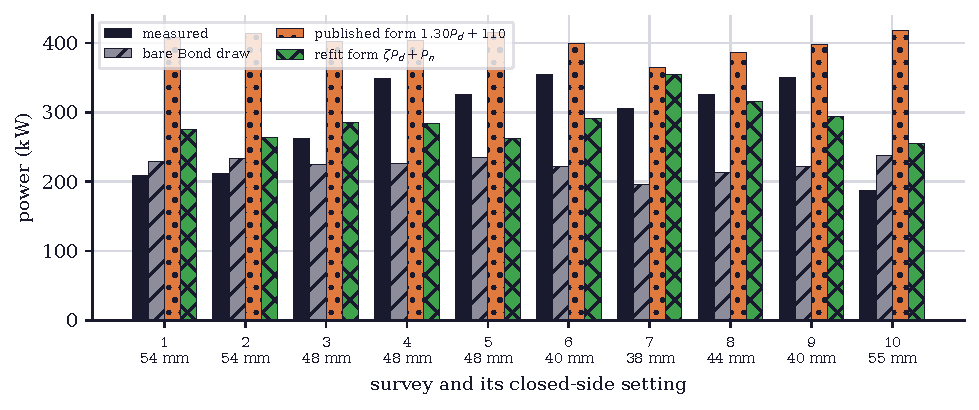
\includegraphics[width=0.9\textwidth]{fig-power-parity.pdf}
\caption{Power per HP500 survey in sample: the measured power, the bare Bond draw of the calibrated engine, the published form
$1.30\,P_d+110$ on that draw and the refit form, with the closed-side setting of each survey under its number.}
\label{fig:power-parity}
\end{figure}

\subsection{Morrell's size-specific crusher energy}\label{sec:m-morrell}

\emph{Theory.} Morrell's method gives the specific energy of comminution circuits from the feed and product sizes and ore work indices
measured by the SMC Test; for a conventional crusher the guideline of the Global Mining Standards and Guidelines Group prints, in its
Annex B (equations B4 and B5)~\cite{gmsg}, following Morrell~\cite{morrell2009},
\begin{align}
W_c &= S_c\,K_2\,M_{ic}\;4\left(x_2^{\,f(x_2)} - x_1^{\,f(x_1)}\right)\ [\mathrm{kWh/t}],\qquad f(x) = -\left(0.295 + \frac{x}{10^{6}}\right),
\label{eq:morrell}\\
S_c &= \min\!\left(1,\ K_s\,(x_1x_2)^{-0.2}\right),\qquad K_s = 55,
\label{eq:sc}
\end{align}
with $x_1$ and $x_2$ the feed and product $80\%$ passing sizes in micrometres, $K_2=1.0$ for a crusher in closed circuit with a
classifying screen ($1.19$ in open circuit) and $M_{ic}$ the crushing work index of the ore in kWh/t. The term $x^{f(x)}$ is a size in
micrometres raised to a small negative power, a pure number, so $W_c$ carries the unit of $M_{ic}$, and the power is $W_c\,Q$ in kW. The
guideline defines the net power as the motor power less the no-load power, so a measured motor power is the net power plus a no-load term.
The primary paper was not opened; the equations are taken from the guideline as printed.

\emph{The fit on the HP500 surveys.} The $M_{ic}$ of the Minas Rio itabirite is not published, so it is a fitted scalar, and so is the
no-load power; both are refit on the nine training surveys of every fold and the held-out survey never enters. The design column of a survey
is $g_i = W_c(M_{ic}=1)\,Q_i$, with the measured $f_{80}$ as $x_1$, the backbone's $P_{80}$ as $x_2$ (a model output used as an input, never as a
target) and the measured feed rate as $Q_i$. Two variants are held out, both closed circuit:
\begin{equation}
\hat P_i = M_{ic}\,g_i \quad\text{(through the origin)},\qquad
\hat P_i = M_{ic}\,g_i + P_{noload} \quad\text{(with a no-load term)},
\label{eq:morrellfit}
\end{equation}
the first fitted by $M_{ic}=\sum g_iP_i/\sum g_i^2$ over the training surveys and the second by ordinary least squares. Their results are in
Section~\ref{sec:results-morrell}: in every fold the variant with a no-load term fits a negative $M_{ic}$.

\emph{The design column on the surveys.} Computed with the product's functions, the specific energy per unit work index,
$W_c(M_{ic}=1)$, lies between $0.058$ (survey 1: $x_1=88{,}000~\mu$m, $x_2=32{,}560~\mu$m, $S_c=0.706$, size term $0.0819$) and $0.069$ (survey 6:
$S_c=0.752$, size term $0.0923$), so the energy law varies by a fifth across the surveys, while the feed rate varies by a factor of two. The design
column $g_i$ therefore follows the feed rate almost exactly (correlation $0.99$, values from $56.4$ to $94.8$~kW per kWh/t), and because the
measured power falls as the feed rate rises, $g_i$ correlates with the measured power at $-0.81$. A positive $M_{ic}$ through the origin can only
scale a column that runs against the target, which is why its error is large; with a free intercept, least squares turns the slope negative.
The diagnosis is the same as for the Bond draw (Section~\ref{sec:m-bond}): both energy laws multiply a specific energy that changes little by a
throughput that changes much, and the measured power does not follow the throughput on these surveys.

\emph{Parameters and how they were set.} $K_s=55$ and $K_2=1.0$ from the guideline; the closed-circuit value is the product's choice, and an
open-circuit factor would only rescale the fitted $M_{ic}$; the two fitted scalars per fold. The exponent $f(x)$ is not constant over crusher sizes: it is $-0.315$ at $20{,}000~\mu$m and $-0.435$ at $140{,}000~\mu$m, so the term
$x^{f(x)}$ falls steeply with size and the size reduction term is dominated by the product size $x_2$. With the sizes of the surveys ($x_1$ from $47{,}000$ to
$140{,}000~\mu$m and $x_2$ from $21{,}230$ to $36{,}600~\mu$m, the backbone's $P_{80}$), $K_s(x_1x_2)^{-0.2}$ is below one, so $S_c$ applies.

\emph{Cost.} $O(1)$ per survey and an $O(n)$ fit per fold. \emph{Assumptions and limits.} Only the conventional-crusher branch of the method
is used: no tumbling-mill terms, no open-circuit $K_2$ in the fit (it would be absorbed by $M_{ic}$), and no size-distribution correction.
The method is not part of the live engine and is not shown as a predictor in the App.

\emph{Implementation and tests.} \texttt{model/\allowbreak{}crusher/\allowbreak{}morrell.py} (\texttt{f\_exponent}, \texttt{size\_term}, \texttt{hardness\_parameter},
\texttt{crusher\_specific\_energy\_kwh\_t}, \texttt{crusher\_power\_kw}) and \texttt{hp500/\allowbreak{}morrell\_fit.py} (\texttt{design\_column},
\texttt{fit\_through\_origin}, \texttt{fit\_with\_no\_load}). The tests check equation B4 against a hand computation, the unit of the result
(linear in $M_{ic}$, kWh/t, times t/h gives kW), the rule on $S_c$, the refusal of non-positive sizes, the recovery of a planted $M_{ic}$ and
no-load power, and that the held-out numbers are reported as they come.

\subsection{The Andersen-Whiten fit calibrated to the HP500 surveys}\label{sec:m-hp500}

\emph{Theory and source.} The one calibrated lane of the product is the secondary cone run with the calibration that Rocha, Campos, Silva and
Tavares published for a Metso HP500 crushing itabirite iron ore~\cite{rocha2024}, at the ten surveys of their Table A1. On this lane the surveys
vary only the setting and the feed $f_{80}$; the throw ($34$~mm) and the speed ($360$~rpm) are machine constants, the feed is rebuilt from the
measured $f_{80}$ as a Rosin-Rammler feed with $n=0.9$, the ore competence is the compact itabirite $A\times b=677.3$ (metadata only, because the
calibrated $t_{10}$ does not use it) and the work index is the blend value $9.0$~kWh/t. The engine then replaces three synthetic relations by the
fitted ones, with sizes in millimetres,
\begin{equation}
K_1 = 0.23\,s + 0.30\,f_{80},\qquad K_2 = \max\!\left(12.0 + 0.55\,s + 0.40\,f_{80},\ 1.05\,K_1\right),\qquad K_3 = 2.3,
\label{eq:hp500class}
\end{equation}
independent of the throw, and
\begin{equation}
t_{10}\,[\%] = 64 - 0.12\,s - 0.23\,f_{80},\qquad Q = Q_T\;\frac{s+T/2}{g_{ref}}\;\sigma_Ne^{1-\sigma_N},\quad Q_T = 647\ \mathrm{t/h},
\label{eq:hp500t10}
\end{equation}
with the power of Equation~\eqref{eq:pc}. The constants are carried from the product's code and its earlier documentation; the publisher page of
the paper refused automated access to every documenting attempt, so their correspondence to the numbered tables of the paper (Tables 1, 4 and 5
in the code's attributions) is not re-verified here.

\emph{The backbone.} The calibrated engine evaluated at each survey is the backbone (Table~\ref{tab:surveys}). Its throughput depends only on the
setting at the fixed throw and speed: from $936.45$~t/h at $38$~mm to $1225.89$~t/h at $55$~mm, linear in the setting. Its product $P_{80}$ ranges
from $21.23$~mm (survey 3) to $36.60$~mm (survey 7), between $0.35$ and $1.1$ times the setting, the physical relation it is graded by since no
size distribution is measured. In sample, the capacity factor of the backbone with the published $Q_T$ reproduces the measured feed rate with a
mean absolute percentage error of $11.55\%$ ($R^2=0.458$). Survey 3 is flagged pass-through and invalid, because its measured $f_{80}$ ($47$~mm)
reads as $47.15$~mm on the grid, below its setting of $48$~mm; it is kept in every evaluation, as a limit of the calibrated lane. The
largest in-sample deviation of the throughput is $26.24\%$ (survey 1, whose measured $1639$~t/h is the largest feed rate of the set).

\emph{The fitted breakage on the surveys.} The fitted $t_{10}$ of Equation~\eqref{eq:hp500t10}, evaluated with the grid $F_{80}$ of each
survey, ranges from $32.1\%$ (survey 7, the coarsest feed, grid $F_{80}=118.9$~mm at a $38$~mm setting) to $47.4\%$ (survey 3, the finest
feed), so the cap of $44\%$ of Section~\ref{sec:m-breakage} binds on two surveys, survey 3 and survey 5 ($44.06\%$, just above it), and on no
other. The coarser the feed, the lower the fitted fineness of the progeny, which is the direction of the fit: the $f_{80}$ coefficient
of $-0.23$ points per millimetre dominates the setting coefficient of $-0.12$ over the range of the surveys. Because the product size is not
measured, none of these values is checked against data; they enter the two measured targets only through the Bond term of the power.

\emph{Parameters and how they were set.} Every constant of Equations~\eqref{eq:hp500class} and~\eqref{eq:hp500t10} is the published fit; the
nominal throw and speed are the product's assumptions (a representative mid-point of the HP500 throw range and the secondary cone's capacity
optimum); the feed exponent is the product's assumption. The calibrated support is the range of the surveys, a setting of $38$ to $55$~mm and a
feed $f_{80}$ of $47$ to $140$~mm; outside it the envelope check flags extrapolation.

\emph{Cost.} One engine evaluation per survey. \emph{Assumptions and limits.} The fit is the paper's: the product holds it to the ten surveys out
of sample and does not perform the calibration. One machine and one ore, so the lane does not transfer.

\emph{Implementation and tests.} \texttt{model/\allowbreak{}crusher/\allowbreak{}hp500.py} (\texttt{HP500\_NOMINAL}, \texttt{Hp500Scalars}, \texttt{operating\_from\_survey}),
\texttt{classification.py} (\texttt{hp500\_params}), \texttt{breakage.py} (\texttt{t10\_calibrated}), \texttt{capacity.py}
(\texttt{HP500\_QREF}) and \texttt{hp500/\allowbreak{}backbone.py}, which writes the backbone document. The acceptance criteria are that the calibrated engine
at each survey equals the backbone document and that the ten surveys are physically plausible to the envelope check
(\texttt{test\_backbone\_is\_the\_engine}, \texttt{test\_envelope\_gate\_the\_ten\_real\_hp500\_surveys\_are\_physically\_plausible}, which
uses a proxy feed and therefore does not see the grid effect of survey 3).

\subsection{The setting-only line}\label{sec:m-line}

\emph{Theory.} The baseline that every other predictor of the surveys is held to is an ordinary least-squares line of one target on the
closed-side setting alone, refit on the training surveys of each fold:
\begin{equation}
\hat y_{t,i} = a_{t,-i} + b_{t,-i}\,s_i,\qquad
\left(a_{t,-i},\,b_{t,-i}\right) = \arg\min_{a,b}\sum_{j\in\mathcal T_{-i}}\left(y_{t,j} - a - b\,s_j\right)^2 ,
\label{eq:line}
\end{equation}
for throughput and for power, with the closed form $b=\sum_j(s_j-\bar s)(y_j-\bar y)/\sum_j(s_j-\bar s)^2$ and $a=\bar y-b\bar s$ over the nine
training surveys. It carries no physics and no engine. Its value is that the claim of any other method is the margin over it: the measured power
correlates with the setting at $-0.82$, so a line on the setting already captures most of what the ten surveys say about power. Fitted on all ten
surveys, the lines are $P = 686 - 8.49\,s$ and $Q = -351 + 31.92\,s$ (Figure~\ref{fig:surveys}), so each millimetre of setting is worth about
$8.5$~kW and $32$~t/h on this machine and ore.

\emph{Held-out residuals in closed form.} For an ordinary least-squares fit the leave-one-out residual has a closed form, which makes
the held-out error of the line transparent. With the leverage of survey $i$ on the setting,
\begin{equation}
h_{ii} = \frac1n + \frac{(s_i-\bar s)^2}{\sum_{j=1}^{n}(s_j-\bar s)^2},\qquad
y_{t,i}-\hat y_{t,i} = \frac{e_{t,i}}{1-h_{ii}},
\label{eq:loo-ols}
\end{equation}
where $e_{t,i}$ is the residual of the line fitted on all ten surveys, the strict held-out residual is the in-sample residual inflated by
$1/(1-h_{ii})$. On the survey table the leverages range from $\levmin$ (the three surveys at $48$~mm, closest to the mean setting of $46.9$~mm) to
$\levmax$ (survey 7 at $38$~mm, the tightest setting); surveys at the ends of the setting range are therefore the ones whose held-out errors grow
most. Evaluating Equation~\eqref{eq:loo-ols} on the table reproduces the document's numbers exactly: an in-sample MAPE of $\lineinP\%$ and a held-out
MAPE of $\linelooP\%$ on power, and $\lineinQ\%$ and $\linelooQ\%$ on throughput, which are the leaky and strict values of Table~\ref{tab:leaky}. The
optimism of the leaky evaluation of the line is thus a pure leverage effect of ten points on one feature, with no fitting freedom to absorb a
survey; the gap of the more flexible predictors in that table is larger because they also absorb part of the held-out survey's noise. These
numbers are computed by \texttt{make\_tables.py} from the survey table, as a check on the protocol, and agree with the committed document.

\emph{Why it is the baseline.} A constant mean ignores the one lever that the surveys vary most, and a free-form fit on the setting and $f_{80}$
spends a second coefficient on a variable that, on these data, adds no held-out skill on power. An exploratory screen of predictor sets on the same
folds, run before the line was added to the product, placed the setting alone ahead of the setting with $f_{80}$, of $1/s$, of the setting with
the measured throughput, and of the measured throughput times the Bond size term; the line was then added as a named predictor with its own
acceptance criterion. The screen is the reason for the choice and not a result of the report, because several forms were tried on ten points.

\emph{Parameters.} Two coefficients per target and fold, both fitted. \emph{Cost.} $O(n)$ per fold. \emph{Assumptions and limits.} Linear in the
setting over $38$ to $55$~mm; it has no meaning outside the surveyed range, and it predicts no product size. Its power coefficient is not a
mechanism: on these surveys the feed rate is set by the plant together with the setting (correlation $+0.81$), so the line on the setting also
carries the effect of the feed rate on power, and a plant that changed the feed rate at a fixed setting would break it. It is a description of
how this machine was operated over the surveyed period, and it is exactly the kind of relation a calibrated mechanistic model must reproduce
before it can claim to add anything.

\emph{Implementation and tests.} \texttt{hp500/\allowbreak{}blin.py} (\texttt{fit\_line}, \texttt{predict\_line}), called by \texttt{hp500/\allowbreak{}loo.py}. The
acceptance criterion is that it reproduces the held-out errors of $12.78\%$ (power) and $13.67\%$ (throughput) of the exploratory screen on the
same folds, and that a survey planted with an absurd target moves every other fold and not its own
(\texttt{test\_b\_lin\_reproduces\_the\_dossier\_numbers}, \texttt{test\_adversarial\_a\_fold\_never\_sees\_its\_held\_out\_survey}).

\subsection{CrusherCal: leave-one-survey-out evaluation with controls and a predictive band}\label{sec:m-crushercal}

\emph{What it is.} CrusherCal is the evaluation protocol of the HP500 lane: the predictors of the two measured targets are fitted and scored on the
same ten folds, with negative controls, a leaky variant to expose optimism, and an $80\%$ predictive band whose coverage is computed out of sample.
It is a protocol and not a predictor of its own; every number it produces is computed from the committed backbone and the survey table.

\emph{The predictors.} For each target, in each fold, on the nine training surveys:
\begin{itemize}
\item \emph{Calibrated backbone.} The engine with its global scalars refit. For throughput, $\hat Q_i=Q_{T,-i}\,\phi_i$ with $\phi_i$ the engine's
capacity factor (the backbone throughput over $647$~t/h) and $Q_{T,-i}=\sum_j\phi_jQ_j/\sum_j\phi_j^2$; for power, the form of
Equation~\eqref{eq:pc} with $(\zeta,P_n)$ refit by ordinary least squares on the Bond draws of the training surveys.
\item \emph{Backbone with a bounded residual.} A ridge regression (penalty $\lambda=1$, intercept not penalised) of the backbone residual on the
standardised setting and $f_{80}$, evaluated at the held-out survey and clipped to $\pm20\%$ of the backbone value, added to the backbone.
\item \emph{Free-form fit.} Ordinary least squares of the raw target on the setting and $f_{80}$, with no physics.
\item The setting-only line (Section~\ref{sec:m-line}) and, for power, the two Morrell variants (Section~\ref{sec:m-morrell}).
\item \emph{Controls.} The constant mean of the training surveys; and a label-shuffle control, the bounded residual trained on the measured values
permuted with a seeded generator, which must not beat the backbone.
\end{itemize}
The ridge fit of the bounded residual and its clipped correction are
\begin{equation}
\hat{\boldsymbol\beta}_{-i}=\left(\mathrm X_{-i}^{\top}\mathrm X_{-i}+\lambda\mathrm D\right)^{-1}\mathrm X_{-i}^{\top}\mathbf r_{-i},\qquad
\hat y^{\mathrm{res}}_{i} = \hat y^{\mathrm{bb}}_{i} + \mathrm{clip}\!\left(\mathbf x_i^{\top}\hat{\boldsymbol\beta}_{-i},\ -0.2\,|\hat y^{\mathrm{bb}}_{i}|,\ 0.2\,|\hat y^{\mathrm{bb}}_{i}|\right),
\label{eq:ridge}
\end{equation}
with $\mathrm X_{-i}$ the standardised setting and $f_{80}$ of the training surveys with a column of ones, $\mathbf r_{-i}$ their backbone
residuals, $\mathrm D$ the identity with a zero in the intercept's position, and $\mathbf x_i$ the held-out survey's row standardised with the
training mean and standard deviation.

\emph{The band.} The $80\%$ interval of the backbone is its prediction plus or minus $1.2816$ standard deviations of its held-out residuals,
\begin{equation}
\hat y_{t,i}\ \pm\ 1.2816\,\sigma_{-i},\qquad
\sigma_{-i}^2 = \frac{1}{n-2}\sum_{j\ne i}\left(r_j - \bar r_{-i}\right)^2,\quad r_j = y_{t,j} - \hat y_{t,j},
\label{eq:band}
\end{equation}
where $r_j$ are the strict held-out residuals and $\sigma_{-i}$ their sample standard deviation over the other nine surveys, so the survey whose
coverage is checked never contributes to its own band (nested coverage). The document also reports the in-sample coverage, in which $\sigma$ comes
from the same ten residuals it is checked against, only to show the difference. The factor $1.2816$ is the two-sided normal quantile of a central
$80\%$ interval. The same nested band, applied to the residuals of the setting-only line and of the free-form fit, gives those predictors the bands
that CrusherBayes is compared with.

\emph{Strict and leaky folds.} Every fit is run twice: strict, on the nine training surveys, and leaky, on all ten including the held-out one. The
difference between the two errors is the optimism of an evaluation that lets a survey into its own fit.

\begin{algorithm}[!t]
\caption{CrusherCal: the strict and leaky leave-one-survey-out evaluation of one target, as \texttt{hp500/\allowbreak{}loo.py} runs it.}
\label{alg:crushercal}
\begin{algorithmic}[1]
\Require surveys $(s_j,f_{80,j},y_j)_{j=1}^{n}$; backbone capacity factors $\phi_j$ or Bond draws $P_{d,j}$; seed $42$
\Ensure held-out predictions of every predictor, their scores, the band and its nested coverage
\State $\tilde{\mathbf y}\gets$ a seeded permutation of $\mathbf y$ \Comment{label-shuffle control}
\For{mode $\in\{$strict, leaky$\}$}
  \For{$i=1$ \textbf{to} $n$}
    \State $\mathcal T\gets\{1..n\}\setminus\{i\}$ if strict, else $\{1..n\}$
    \State fit the backbone scalars on $\mathcal T$; $\hat y^{\mathrm{bb}}_i\gets$ backbone at survey $i$
    \State fit the ridge residual on $\mathcal T$; $\hat y^{\mathrm{res}}_i\gets\hat y^{\mathrm{bb}}_i+\mathrm{clip}(\hat r_i,\pm0.2\,|\hat y^{\mathrm{bb}}_i|)$
    \State fit the free-form fit, the setting-only line and, for power, both Morrell variants on $\mathcal T$; predict survey $i$
    \State $\hat y^{\mathrm{mean}}_i\gets$ mean of $y$ over $\mathcal T$; refit the residual on $\tilde{\mathbf y}$ for the control
  \EndFor
  \State score every predictor: MAPE, RMSE, $R^2$, largest deviation
\EndFor
\State $r_j\gets y_j-\hat y^{\mathrm{bb}}_j$ (strict); for each $i$: $\sigma_{-i}\gets\mathrm{sd}(r_{j\ne i})$, covered$_i\gets|r_i|\le1.2816\,\sigma_{-i}$
\State \Return predictions, scores, $\sigma$, half-width, in-sample and nested coverage
\end{algorithmic}
\end{algorithm}

\emph{Parameters and how they were set.} The clip fraction $0.20$ (a physical bound on a correction to a physics prediction), the ridge penalty
$1.0$ (to keep a fit on nine points humble), the seed $42$; all three were set before the first run and are recorded in the document. The
expectation stated before the run was that the bounded residual would give a marginal or null improvement over the backbone; Section~\ref{sec:results}
reports what came out. \emph{Cost.} Per target and mode, $n$ least-squares fits of at most three coefficients for each predictor; the engine is
evaluated once per survey, by the backbone, and not inside the folds. \emph{Limits.} With $n=10$, one survey moves a coverage by $0.1$, and a difference below about three points of MAPE is within noise;
the protocol is not a significance test.

\emph{Implementation and tests.} \texttt{hp500/\allowbreak{}loo.py} (\texttt{fold\_indices}, \texttt{fit\_capacity\_base}, \texttt{fit\_power\_form},
\texttt{fit\_residual}, \texttt{fit\_freeform}, \texttt{predictive\_band}, \texttt{nested\_band\_coverage}, \texttt{band\_factor}). The acceptance
criteria are that the label-shuffle control does not beat the backbone, that the backbone beats the constant mean on throughput, that the
leaky-strict gap is exposed and that the band's coverage is reported (\texttt{test\_adversarial\_the\_label\_shuffle\_control\_does\_not\_beat\_the\_backbone},
\texttt{test\_tph\_backbone\_has\_real\_skill}, \texttt{test\_adversarial\_the\_leaky\_folds\_expose\_the\_optimism\_gap}).

\subsection{The envelope check}\label{sec:m-envelope}

\emph{Principle.} An empirical model must flag implausible and out-of-calibration inputs and never answer them with a confident number. The envelope
check applies five rules to an operating point and the feed size the engine reads; it is also the baseline of the anomaly slot, the answer given when
no valid autoencoder is released.

\emph{Rules.} Writing $\mathbb 1[\cdot]$ for an indicator, the point is implausible, and therefore invalid, when
\begin{equation}
\iota(\mathbf u) = \mathbb 1[s\le0]\ \lor\ \mathbb 1[x_{63}\le0]\ \lor\ \mathbb 1[F_{80}>0\ \land\ s\ge F_{80}],
\label{eq:implausible}
\end{equation}
with the codes \texttt{css\_nonpositive}, \texttt{feed\_nonpositive} and \texttt{f80\_lt\_css}; and a point on the calibrated lane is extrapolating,
without being invalid, when
\begin{equation}
\xi(\mathbf u) = \mathbb 1[s\notin[38,55]\ \mathrm{mm}]\ \lor\ \mathbb 1[F^{\mathrm{decl}}_{80}\notin[47,140]\ \mathrm{mm}],
\label{eq:extrapolating}
\end{equation}
with the codes \texttt{css\_outside\_calibrated} and \texttt{f80\_outside\_calibrated}, where $F^{\mathrm{decl}}_{80}=x_{63}(\ln5)^{1/n}$ is the
declared feed size rounded to a micrometre (the untruncated value, so that a feed coarser than the grid is judged by its own size and a survey on
the $140$~mm edge is not pushed over it by round-off). The calibrated support is the range of the ten surveys of Rocha et al.~\cite{rocha2024}.

\emph{Sourced warnings.} Two further codes run after the check in both engines on the operating point and the computed reduction ratio. A setting
below the vendor minimum of the machine class writes \texttt{css\_below\_vendor\_minimum}: $16$~mm for the secondary cone (Metso HP500 standard
liners), $6$~mm for the tertiary and short-head cones (HP500 short head)~\cite{metsoHP}, $40$~mm for the jaw (the smallest minimum of the Nordberg
C Series)~\cite{metsoC}, and none for the gyratory, for which no source was found, so the check is skipped rather than guessed. A reduction ratio
$F_{80}/P_{80}$ above the typical ceiling of one stage writes \texttt{reduction\_ratio\_above\_typical}: $5$ for the HP standard chamber, $4$ for
the short-head chamber~\cite{metsoHP}, and $4$ for the jaw and the gyratory~\cite{metsoBasics}. Both bounds are strict and both are warnings: they
never change the validity, because the vendor calls the minimum setting soft (the setting at which the crusher runs without ring bounce, which can
change with the rock) and the ratios are typical ranges, not maxima. Of the seventeen circuit cases, CK1, S05, S06, T01, T02, H01 and H02 carry the
ratio warning and S06, at $12$~mm, also the setting warning; the ten surveys carry neither.

\emph{Committed behaviour.} The controls CI1 and CP1, the gyratory case G02 and the survey HP500-03 carry \texttt{f80\_lt\_css} and are invalid. On the
synthetic lane the check flags only implausible inputs, so a plausible point outside the training range of the learned models passes it; the
autoencoder (Section~\ref{sec:m-ae}) scores distance from the training manifold, the complementary check.

\emph{Why the declared size.} The extrapolation rule of Equation~\eqref{eq:extrapolating} tests the declared feed size and not the grid value
because the two differ for coarse feeds: a feed with a declared $F_{80}$ of $180$~mm and the exponent $0.9$ of the survey feeds reads $135.8$~mm on the $256$~mm grid, inside the
calibrated support, and testing the grid value would let a feed coarser than any survey pass as supported. The rounding to a micrometre is there
because the feed of a survey is rebuilt from its $f_{80}$ by the inverse of Equation~\eqref{eq:rr}, and the floating-point round trip can return
a value a few units in the last place above $140$~mm for the survey on the edge of the support. The implausibility rule, in contrast, uses the grid value, because it asks
whether the engine itself can grip the feed it works with.

\emph{What the check does not see.} On the synthetic lane the check knows three implausibility rules and nothing about the ranges over which the
learned models were trained, so a secondary cone at a $90$~mm setting with a plausible feed passes it while lying at the edge of the surrogate's
training range; the applicability rule of the model slots (Section~\ref{sec:m-surrogate}) and the autoencoder score handle that case.

\emph{Cost.} $O(1)$. \emph{Limits.} Five rules and two warnings, not the distribution of the data; a point that passes is not thereby accurate.

\emph{Implementation and tests.} \texttt{model/\allowbreak{}crusher/\allowbreak{}envelope.py} (\texttt{check\_envelope}, \texttt{HP500\_ENVELOPE\_CSS\_MM},
\texttt{HP500\_ENVELOPE\_F80\_MM}) and \texttt{model/\allowbreak{}crusher/\allowbreak{}bounds.py} (\texttt{check\_bounds}). The acceptance criteria are that an implausible
point is flagged and invalid and that a calibrated point outside the support is flagged as extrapolating
(\texttt{test\_envelope\_gate\_an\_implausible\_point\_is\_flagged\_and\_marked\_invalid},
\texttt{test\_envelope\_gate\_calibrated\_lane\_flags\_out\_of\_support\_as\_extrapolating}); further tests cover the strict bounds, the gyratory skip
and the unchanged validity of the warnings.
